\documentclass{scrartcl}
\usepackage[letterpaper,top=1in,bottom=1in]{geometry}
% \usepackage{tabulary}
\usepackage[american]{babel}
% \usepackage{booktabs}
\usepackage{csquotes}
\usepackage{fontspec}
\usepackage{graphicx}
\usepackage{hyperref}
\usepackage{listings}
\usepackage{siunitx}
\usepackage{svg}
\usepackage{scrlayer-fancyhdr}
\usepackage{scrextend}
\usepackage{tabularray}
\usepackage{wrapfig}
\usepackage{subcaption}

\title{CMSC 315, Project 2}
\author{Alberth Matos}
\date{3 Feb 2026}
\UseTblrLibrary{booktabs}
\setmainfont{Hoefler Text}
\setmonofont{Courier Prime}
\setlength\heavyrulewidth{0.20ex}
\setlength\cmidrulewidth{0.10ex}
\setlength\lightrulewidth{0.10ex}
\newcolumntype{L}{>{\raggedright\arraybackslash}X} % Defines new column type
% with variable length, similar to X in tabularx, but is left aligned rather
% than justified
\newcolumntype{R}{>{\raggedleft\arraybackslash}X} % Defines new column type
% with variable length, similar to X in tabularx, but is right aligned rather
% than justified
\newcolumntype{C}{>{\centering\arraybackslash}X} % Defines new column type
% with variable length, similar to X in tabularx, but is centered rather
% than justified
\hypersetup{
    pdftitle={\@title},
    pdfauthor={\@author}
}
\lstdefinestyle{numberedLines}{
    numbers=left,
    numberstyle=\small,
    stepnumber=1,
    numbersep=5pt,
    frame=none,
    framerule=0.5pt,
    framesep=2pt,
    basicstyle=\ttfamily,
    keywordstyle=\color{blue}\bfseries,
    commentstyle=\color{gray},
    stringstyle=\color{black},
    showstringspaces=false,
    breaklines=true,
    postbreak=\raisebox{0ex}[0ex][0ex]{\ensuremath{\hookrightarrow\space}}
}
\lstset{style=numberedLines}
\setcounter{page}{1}

\pagestyle{fancy}
\fancyhead{}
\fancyfoot{}
\fancyhead[R]{A.Matos}
\fancyhead[L]{CMSC 315, Project 2}
\fancyfoot[C]{\thepage}

\begin{document}
\maketitle
\tableofcontents
\thispagestyle{empty}
\newpage
\section{Design}
The goal of the project was to implement \emph{Natural Language Processing}
(NLP) utility methods to analyze a paragraph of text entered by the user,
including word frequency and sentiment analysis.  The project also required
us to create unit tests for each method created, ensuring that the methods
function correctly and efficiently.

\subsection{UML Diagram}
\includesvg{WordFrequency-and-SentimentAnalysis.svg}
\newpage
\section{Testing:}
\subsection{Test Plan}
\begin{enumerate}
	\item Unit tests for each method in NLPUtils.java
	\item Test sentences for full application validation.
	      \begin{enumerate}
		      \item \enquote{WOW!?!    That .?\# is REALLY(reaLLy) amazing!      }\label{sentence1}
		      \item \enquote{This is a test sentence. This is a great test sentence.  This awful test sentence.  Many sentences.}\label{sentence2}
		      \item \enquote{I love dancing in the rain like it’s the most magical thing in existence, adore sunsets that explode with color, like spontaneous road trips, yet I hate traffic jams with every ounce of my being, despise burnt toast, and worship the rare, mind-blowingly perfect moments that make life feel impossibly, overwhelmingly extraordinary.}\footnote{Indicated sentences generated with ChatGPT.\label{chatGPT}}\label{sentence3}
		      \item \enquote{I absolutely love the smell of rain like it’s the most divine perfume on the planet, yet I utterly hate stepping in puddles as if the universe itself is conspiring against me. I adore sunrises with a passion that could light cities, and I love coffee so intensely it feels like a life force flowing through my veins. I like quiet mornings, but I love thunderous storms more than anything else imaginable.}\footref{chatGPT}\label{sentence4}
		      \item \enquote{I love a good BOOK and LOVE sad BooK book!}\label{sentence5}
		      \item \enquote{I really love a good book, and You REALLY love a sad movie. We both ReAllY LOVE going for a walk!}\label{sentence6}
		      \item \enquote{SO is.! It????}\label{sentence7}
	      \end{enumerate}
\end{enumerate}
\newpage
\subsection{Test Results}
\subsubsection{Test 1, Unit Tests}
Please note, unit tests were executed using JUnit.  The NLPUtilityTest class
is included here in Section \ref{sec:unittests}.  Please reference the
NLPUtilityTest class for details on what each unit test verifies.
\newline
\begin{wrapfigure}{r}{0.6\textwidth}
	\fbox{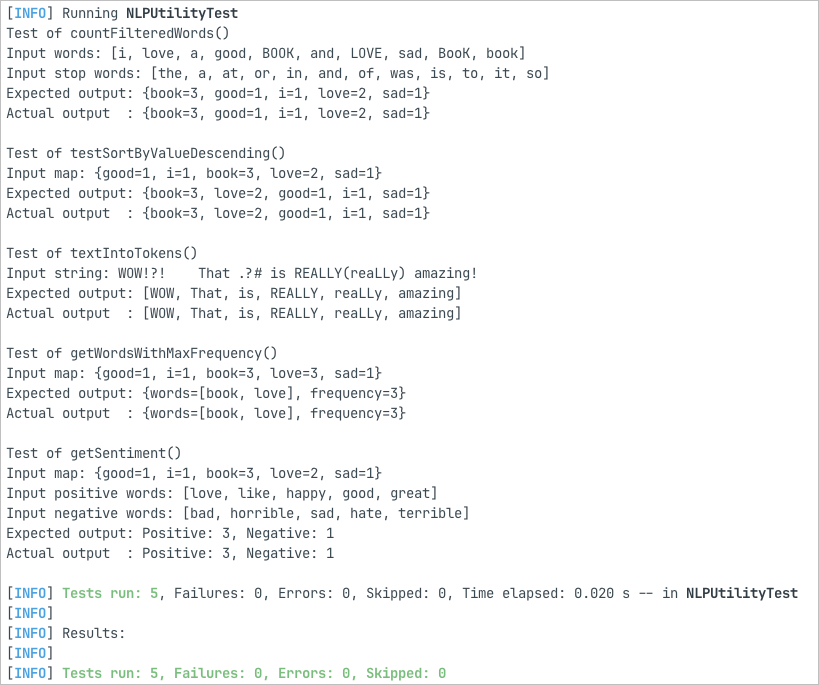
\includegraphics[width=1.0\linewidth]{images/unittests.png}}
	\caption{Unit Tests, via JUnit}
\end{wrapfigure}
Expected output:\newline
\begin{lstlisting}
 Running NLPUtilityTest
 Tests run: 5, Failures: 0, Errors: 0, Skipped: 0, Time elapsed: 0.023 s -- in NLPUtilityTest

 Results:

 Tests run: 5, Failures: 0, Errors: 0, Skipped: 0
\end{lstlisting}

\clearpage
\subsubsection{Test 2, Sentence \ref{sentence1}}
\begin{wrapfigure}{r}{0.4\textwidth}
	\fbox{
\includegraphics[width=1.0\linewidth]{images/test1.png}}
	\caption{Sentence \ref{sentence1} image}
\end{wrapfigure}
Expected output:\newline
\begin{lstlisting}
Tokenized:
[WOW, That, is, REALLY, reaLLy, amazing]

Word map sorted by key ascending:
amazing:1
really:2
that:1
wow:1

Word map sorted by value descending:
really:2
amazing:1
that:1
wow:1

Sentiment: Positive: 0, Negative: 0

Most frequent word(s): [really] (used 2 times)
\end{lstlisting}

\clearpage
\subsubsection{Test 3, Sentence \ref{sentence2}}
\begin{wrapfigure}{r}{0.6\textwidth}
	\fbox{
\includegraphics[width=1.0\linewidth]{images/test2.png}}
	\caption{Sentence \ref{sentence2} image}
\end{wrapfigure}
Expected output:\newline
\begin{lstlisting}
Tokenized:
[This, is, a, test, sentence, This, is, a, great, test, sentence, This, awful, test, sentence, Many, sentences]

Word map sorted by key ascending:
awful:1
great:1
many:1
sentence:3
sentences:1
test:3
this:3

Word map sorted by value descending:
sentence:3
test:3
this:3
awful:1
great:1
many:1
sentences:1

Sentiment: Positive: 1, Negative: 0

Most frequent word(s): [sentence, test, this] (used 3 times)
\end{lstlisting}

\clearpage
\subsubsection{Test 4, Sentence \ref{sentence3}}
\begin{wrapfigure}{r}{0.6\textwidth}
	\fbox{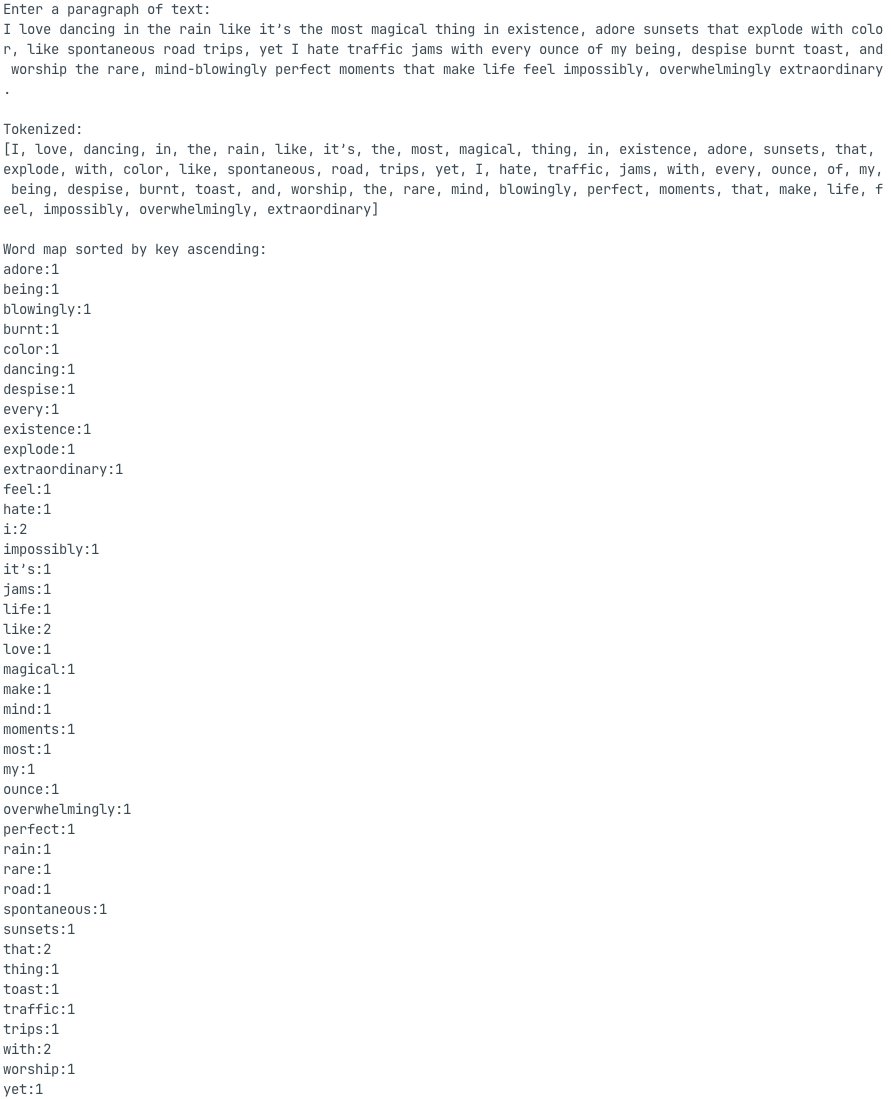
\includegraphics[width=1.0\linewidth]{images/test3-1.png}}
	\fbox{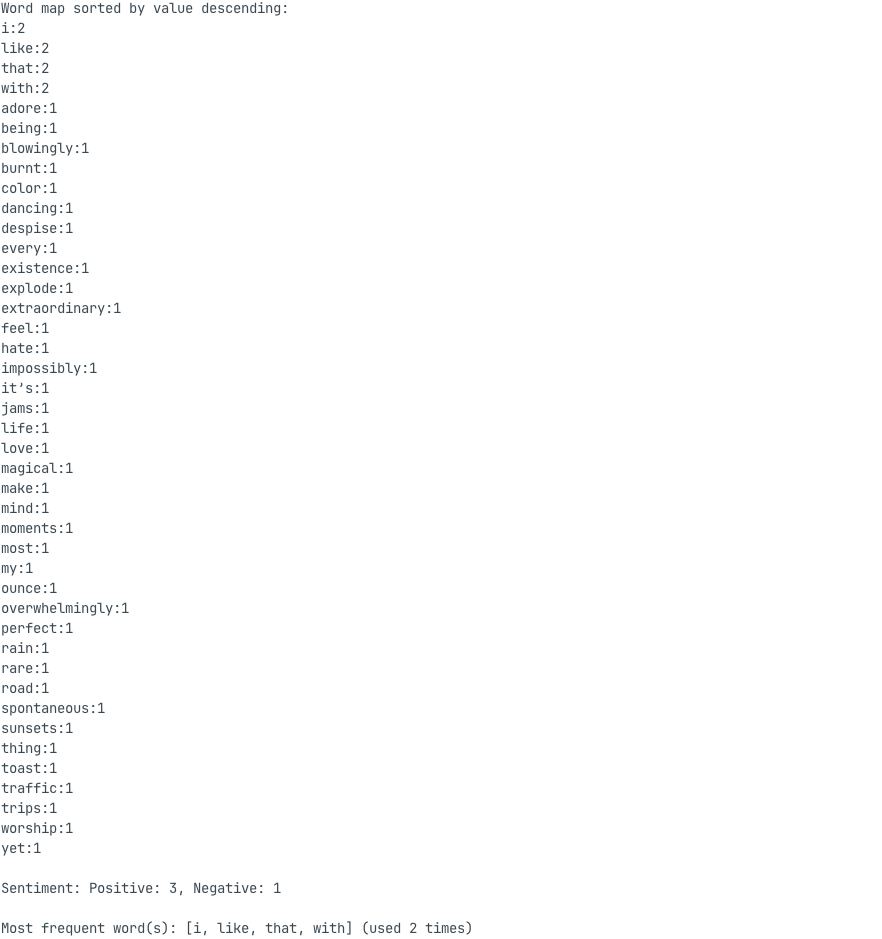
\includegraphics[width=1.0\linewidth]{images/test3-2.png}}
	\caption{Sentence \ref{sentence3} images}
\end{wrapfigure}
Expected output:\newline
\begin{lstlisting}
Tokenized:
[I, love, dancing, in, the, rain, like, it’s, the, most, magical, thing, in, existence, adore, sunsets, that, explode, with, color, like, spontaneous, road, trips, yet, I, hate, traffic, jams, with, every, ounce, of, my, being, despise, burnt, toast, and, worship, the, rare, mind, blowingly, perfect, moments, that, make, life, feel, impossibly, overwhelmingly, extraordinary]

Word map sorted by key ascending:
adore:1
being:1
blowingly:1
burnt:1
color:1
dancing:1
despise:1
every:1
existence:1
explode:1
extraordinary:1
feel:1
hate:1
i:2
impossibly:1
it’s:1
jams:1
life:1
like:2
love:1
magical:1
make:1
mind:1
moments:1
most:1
my:1
ounce:1
overwhelmingly:1
perfect:1
rain:1
rare:1
road:1
spontaneous:1
sunsets:1
that:2
thing:1
toast:1
traffic:1
trips:1
with:2
worship:1
yet:1

Word map sorted by value descending:
i:2
like:2
that:2
with:2
adore:1
being:1
blowingly:1
burnt:1
color:1
dancing:1
despise:1
every:1
existence:1
explode:1
extraordinary:1
feel:1
hate:1
impossibly:1
it's:1
jams:1
life:1
love:1
magical:1
make:1
mind:1
moments:1
most:1
my:1
ounce:1
overwhelmingly:1
perfect:1
rain:1
rare:1
road:1
spontaneous:1
sunsets:1
thing:1
toast:1
traffic:1
trips:1
worship:1
yet:1

Sentiment: Positive: 3, Negative: 1

Most frequent word(s): [i, like, that, with] (used 2 times)
\end{lstlisting}

\clearpage
\subsubsection{Test 5, Sentence \ref{sentence4}}
Expected output:\newline
\begin{lstlisting}
Tokenized:
[I, absolutely, love, the, smell, of, rain, like, it’s, the, most, divine, perfume, on, the, planet, yet, I, utterly, hate, stepping, in, puddles, as, if, the, universe, itself, is, conspiring, against, me, I, adore, sunrises, with, a, passion, that, could, light, cities, and, I, love, coffee, so, intensely, it, feels, like, a, life, force, flowing, through, my, veins, I, like, quiet, mornings, but, I, love, thunderous, storms, more, than, anything, else, imaginable]
Word map sorted by key ascending:
absolutely:1
adore:1
against:1
anything:1
as:1
but:1
cities:1
coffee:1
conspiring:1
could:1
divine:1
else:1
feels:1
flowing:1
force:1
hate:1
i:6
if:1
imaginable:1
intensely:1
itself:1
it's:1
life:1
light:1
like:3
love:3
me:1
more:1
mornings:1
most:1
my:1
on:1
passion:1
perfume:1
planet:1
puddles:1
quiet:1
rain:1
smell:1
stepping:1
storms:1
sunrises:1
than:1
that:1
through:1
thunderous:1
universe:1
utterly:1
veins:1
with:1
yet:1

Word map sorted by value descending:
i:6
like:3
love:3
absolutely:1
adore:1
against:1
anything:1
as:1
but:1
cities:1
coffee:1
conspiring:1
could:1
divine:1
else:1
feels:1
flowing:1
force:1
hate:1
if:1
imaginable:1
intensely:1
itself:1
it’s:1
life:1
light:1
me:1
more:1
mornings:1
most:1
my:1
on:1
passion:1
perfume:1
planet:1
puddles:1
quiet:1
rain:1
smell:1
stepping:1
storms:1
sunrises:1
than:1
that:1
through:1
thunderous:1
universe:1
utterly:1
veins:1
with:1
yet:1

Sentiment: Positive: 6, Negative: 1

Most frequent word(s): [i] (used 6 times)
\end{lstlisting}

\begin{figure}
	\centering
	\begin{subfigure}{0.494\textwidth}
		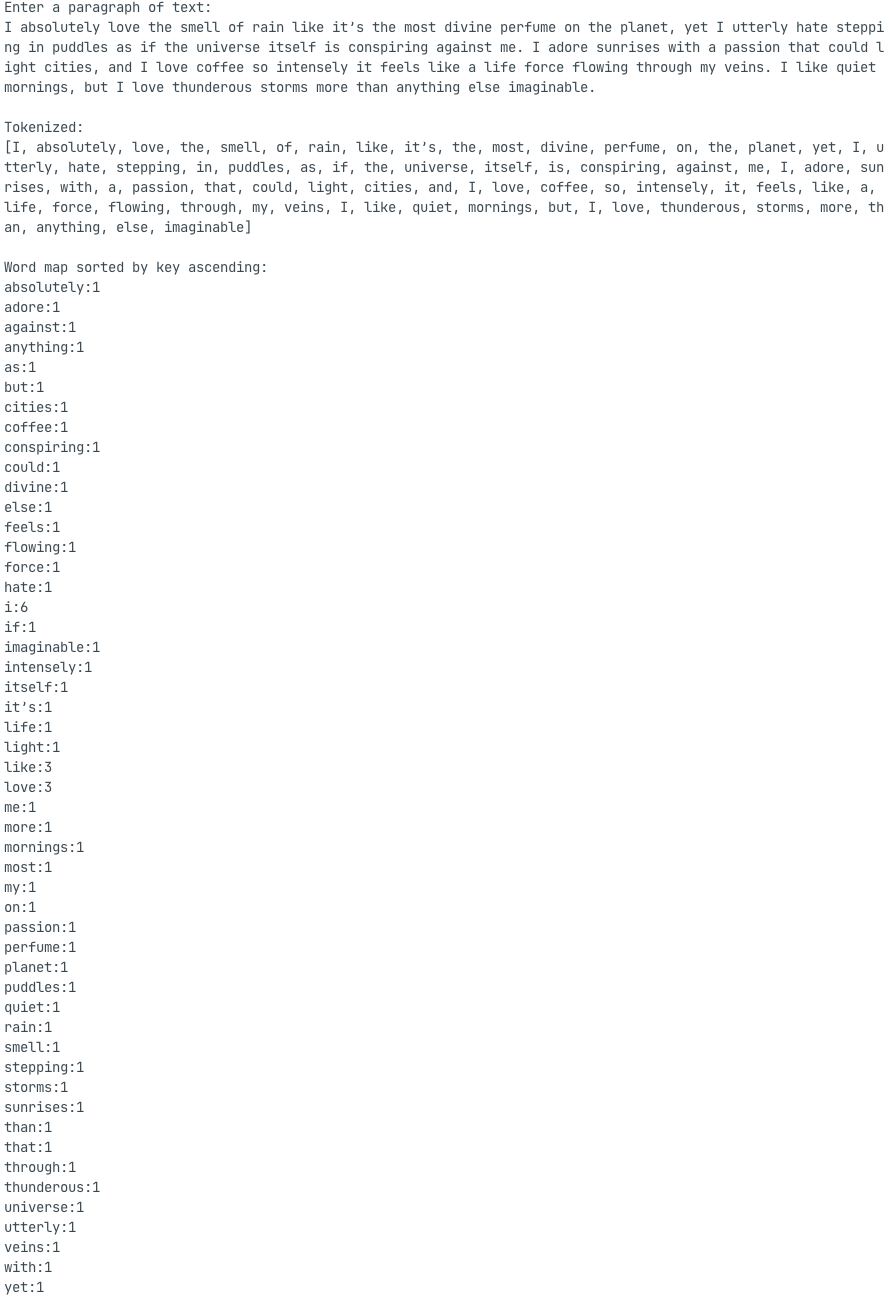
\includegraphics[width=1.0\linewidth]{images/test4-1.png}
		\caption{Sentence \ref{sentence4} image 1}
	\end{subfigure}
	\begin{subfigure}{0.494\textwidth}
		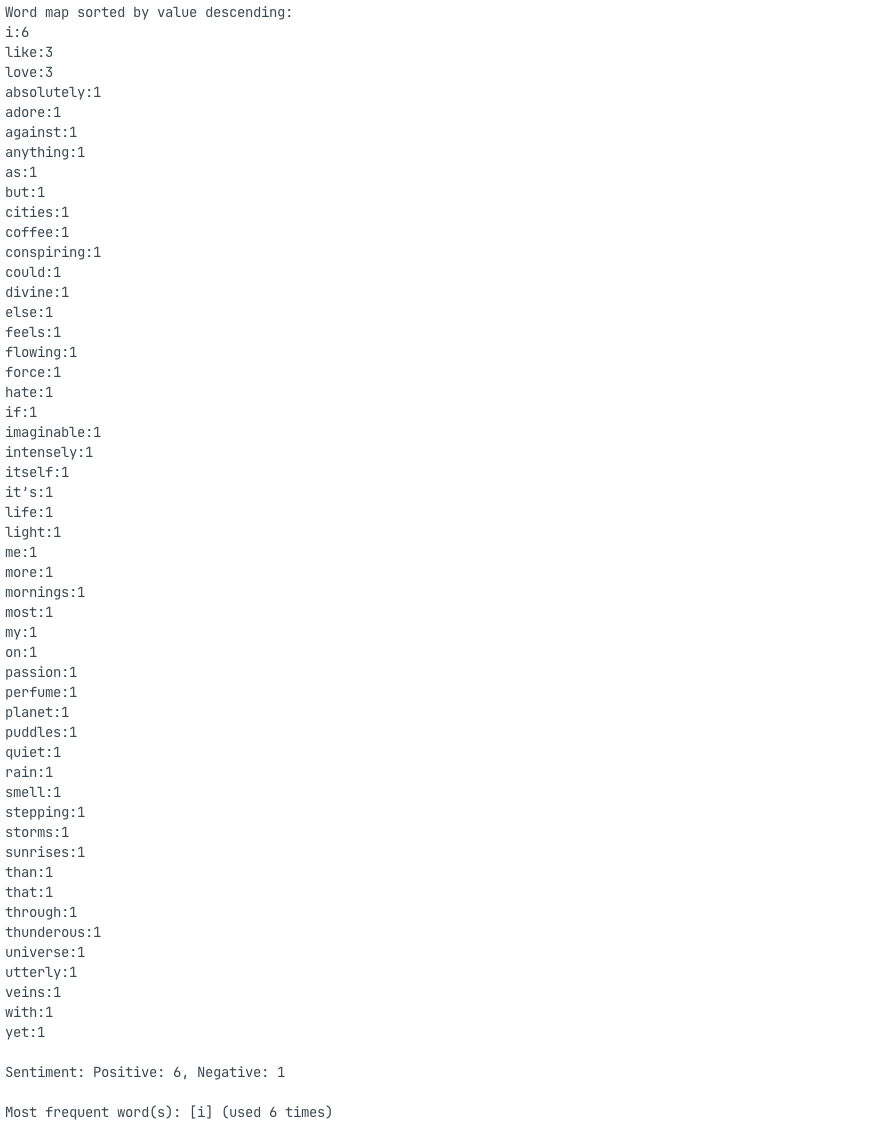
\includegraphics[width=1.0\linewidth]{images/test4-2.png}
		\caption{Sentence \ref{sentence4} image 2}
	\end{subfigure}
\end{figure}

\clearpage
\subsubsection{Test 6, Sentence \ref{sentence5}}
\begin{wrapfigure}{r}{0.4\textwidth}
	\fbox{
\includegraphics[width=1.0\linewidth]{images/test5.png}}
	\caption{Sentence \ref{sentence5} image}
\end{wrapfigure}
Expected output:\newline
\begin{lstlisting}
Tokenized:
[I, love, a, good, BOOK, and, LOVE, sad, BooK, book]

Word map sorted by key ascending:
book:3
good:1
i:1
love:2
sad:1

Word map sorted by value descending:
book:3
love:2
good:1
i:1
sad:1

Sentiment: Positive: 3, Negative: 1

Most frequent word(s): [book] (used 3 times)
\end{lstlisting}

\clearpage
\subsubsection{Test 7, Sentence \ref{sentence6}}
\begin{wrapfigure}{r}{0.6\textwidth}
	\fbox{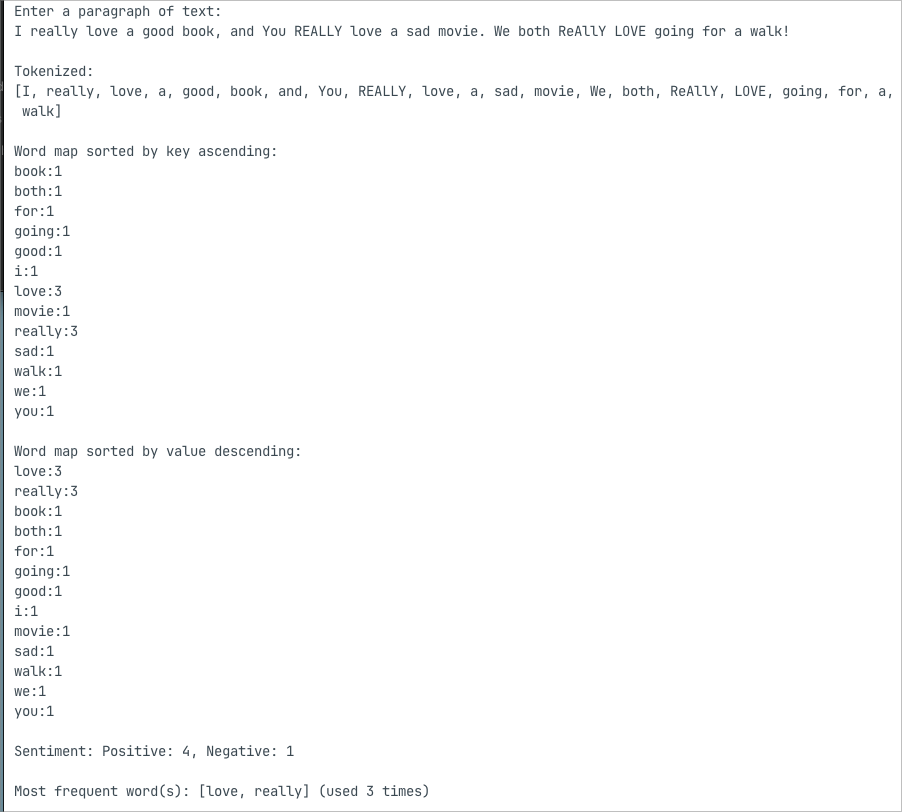
\includegraphics[width=1.0\linewidth]{images/test6.png}}
	\caption{Sentence \ref{sentence6} image}
\end{wrapfigure}
Expected output:\newline
\begin{lstlisting}
Tokenized:
[I, really, love, a, good, book, and, You, REALLY, love, a, sad, movie, We, both, ReAllY, LOVE, going, for, a, walk]

Word map sorted by key ascending:
book:1
both:1
for:1
going:1
good:1
i:1
love:3
movie:1
really:3
sad:1
walk:1
we:1
you:1

Word map sorted by value descending:
love:3
really:3
book:1
both:1
for:1
going:1
good:1
i:1
movie:1
sad:1
walk:1
we:1
you:1

Sentiment: Positive: 4, Negative: 1

Most frequent word(s): [love, really] (used 3 times)
\end{lstlisting}

\clearpage
\subsubsection{Test 8, Sentence \ref{sentence7}}
\begin{wrapfigure}{r}{0.4\textwidth}
	\fbox{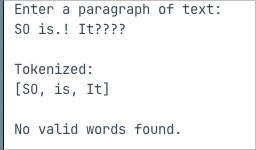
\includegraphics[width=1.0\linewidth]{images/test7.png}}
	\caption{Sentence \ref{sentence7} image}
\end{wrapfigure}
Expected output:\newline
\begin{lstlisting}
Tokenized:
[SO, is, It]

No valid words found.
\end{lstlisting}

\clearpage
\section{Lessons Learned}
The single most important lesson learned from the project was the importance
of reading the requirements carefully and thoroughly, especially when
the answers to one's question may well be answered within the offered examples.

For this particular project, it was ambiguous to this programmer whether the
\emph{testSortByValueDescending()} method should, in addition to its main
purpose of sorting by value in descending order, also sort by key.  To this
programmer, performing the additional sort by key provided a more accurate
representation of the data, and appealed to my inner sense of order.  While
it was not required in the documentation, careful observation of the
\emph{Sample Program Flow} and \emph{Empty or Non-Meaningful Input} examples
showed the same behavior.
\newpage
\section{Unit Tests}
\label{sec:unittests}
\lstinputlisting[language=Java]{../src/test/java/NLPUtilityTest.java}
\end{document}
